% !TEX root = main.tex
%Yael participó en esto.
\noindent
\section{Actividad práctica III} \sangria{} Se conformó un circuito en protoboard, aprovechando que este ya fue analizado y simulado. El objetivo de esta sección es verificar las mediciones calculadas usando un multímetro.
\subsection{Procedimiento del armado del circuito y mediciones}
\begin{enumerate} 
    \item Armar en protoboard el circuito de referencia:
    \begin{center}
        \tikzset{
          hole/.style = {fill = #1, circle, minimum width = 1mm, inner sep = 0mm},
          wire/.style = {draw = #1, line width = 0.2mm},
          label/.style = {rotate = 0, black!50!white, font=\sffamily, anchor = center},
            resistor/.style= {rectangle, draw=black, minimum width=6mm, minimum height=2mm, fill=orange!30}

        }
        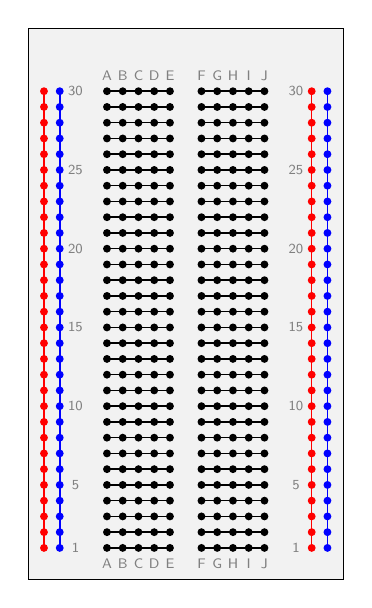
\begin{tikzpicture}[x=2mm,y=2mm]
          \draw[fill=black!05!white] (-4,-1) rectangle (16,34);
          
          \draw[wire=red]  (-3,1) -- (-3,30);
          \draw[wire=blue] (-2,1) -- (-2,30);
          \draw[wire=red]  (14,1) -- (14,30);
          \draw[wire=blue] (15,1) -- (15,30);
          
          \foreach \yi in {1,...,30}{
            \node[hole=red]  at (-3,\yi){};
            \node[hole=blue] at (-2,\yi){};
            \node[hole=red]  at (14,\yi){};
            \node[hole=blue] at (15,\yi){};

            \foreach \xs in {0,6}{
              \draw[wire=black] (1+\xs,\yi) -- (5+\xs,\yi);
              \foreach \xi in {1,2,3,4,5}{
                \node[hole=black] at (\xi+\xs,\yi){};
              }
            }
          }

          \foreach \m/\xi in {A/1,B/2,C/3,D/4,E/5,F/7,G/8,H/9,I/10,J/11}{
            \node[label=0] at (\xi, 0) {\tiny\m};
            \node[label=0] at (\xi,31) {\tiny\m};
          }

          \foreach \n/\yi in {1,5,10,15,20,25,30}{
            \node[label=0] at (-1,\yi) {\tiny\n};
            \node[label=0] at (13,\yi) {\tiny\n};
          }
          % \draw[wire=black] (1,22) -- (1,30);
          % \node[resistor] at (1,26) {R1};

          % \draw[wire=black] (2,22) -- (2,30);
          % \node[resistor] at (2,26) {R2};

          % \draw[wire=black] (10,22) -- (15,22);
          % \node[resistor, rotate=90] at (13,22) {R3};
        \end{tikzpicture}
\end{center}
        \imagen{7cm}{./imagenes/protoSuperior.jpg}
        \begin{center} \textbf{Circuito protoboard - vista superior} \end{center}
        \imagen{7cm}{./imagenes/protoZoom.jpg}
        \begin{center} \textbf{Circuito protoboard - enfoque resistencias} \end{center}
        \resistencia{brown}{black}{orange}{gold} $\rightarrow 10k\Omega$
        \resistencia{orange}{orange}{red}{gold} $\rightarrow 4,7k\Omega$
        \resistencia{yellow}{violet}{red}{gold} $\rightarrow 3,3k\Omega$
\end{enumerate}
\saltoPag{}
\begin{enumerate}[resume]
    \item Ajustar la tensión de la fuente de alimentación a la tensión especificada: 
        \imagen{5cm}{./imagenes/tensionReal.jpg}
    \item Tomar y comparar los elementos del circuito con las magnitudes calculadas y las simuladas: \\[10pt]

        \begin{minipage}{\textwidth}
            \hspace{-1cm}
            \scriptsize
            \begin{tabular}{| p{1cm} p{1cm} p{1cm} p{1cm} p{1cm} p{1cm} |}
                \hline
                \multicolumn{1}{|m{1.4cm}}{\centering\textbf{Magnitud}} &
                \multicolumn{1}{m{1.4cm}}{\centering\textbf{Concepto}} &
                \multicolumn{1}{m{1cm}}{\centering\textbf{$V_S$}} &
                \multicolumn{1}{m{1cm}}{\centering\textbf{$R_1$}} &
                \multicolumn{1}{m{1cm}}{\centering\textbf{$R_2$}} &
                \multicolumn{1}{m{1cm}|}{\centering\textbf{$R_3$}} \\
                \hline
                \multicolumn{1}{|m{1.4cm}}{\multirow{3}{*}{\centering\textbf{Tensión}}} &
                \multicolumn{1}{m{1.4cm}}{\centering\textbf{Análisis}} &
                \multicolumn{1}{m{1cm}}{\centering$10V$} &
                \multicolumn{1}{m{1cm}}{\centering$\frac{80000}{9551}V$} &
                \multicolumn{1}{m{1cm}}{\centering$\frac{15510}{9551}V$} &
                \multicolumn{1}{m{1cm}|}{\centering$\frac{15510}{9551}V$} \\
                                                      &
                \multicolumn{1}{m{1.4cm}}{\textbf{Simulación}} &
                \multicolumn{1}{m{1cm}}{\centering$10V$} &
                \multicolumn{1}{m{1cm}}{\centering$8,37V$} &
                \multicolumn{1}{m{1cm}}{\centering$1,62V$} &
                \multicolumn{1}{m{1cm}|}{\centering$1,62V$} \\
                                                      &
                \multicolumn{1}{m{1.4cm}}{\centering\textbf{Medición [esc. 60V]}} &
                \multicolumn{1}{m{1cm}}{\centering$9,98V$} &
                \multicolumn{1}{m{1cm}}{\centering$8,38V$} &
                \multicolumn{1}{m{1cm}}{\centering$1,60V$} &
                \multicolumn{1}{m{1cm}|}{\centering$1,60V$} \\
                \hline
                \multicolumn{1}{|m{1.4cm}}{\multirow{3}{*}{\centering\textbf{Corriente}}} &
                \multicolumn{1}{m{1.4cm}}{\centering\textbf{Análisis}} &
                \multicolumn{1}{m{1cm}}{\centering$\frac{8}{9551}A$} &
                \multicolumn{1}{m{1cm}}{\centering$\frac{8}{9551}A$} &
                \multicolumn{1}{m{1cm}}{\centering$\frac{33}{95510}A$} &
                \multicolumn{1}{m{1cm}|}{\centering$\frac{47}{95510}A$} \\
                                                      &
                \multicolumn{1}{m{1.4cm}}{\textbf{Simulación}} &
                \multicolumn{1}{m{1cm}}{\centering$-0,837mA$} &
                \multicolumn{1}{m{1cm}}{\centering$0,837mA$} &
                \multicolumn{1}{m{1cm}}{\centering$0,345mA$} &
                \multicolumn{1}{m{1cm}|}{\centering$0,492mA$} \\
                                                      &
                \multicolumn{1}{m{1.4cm}}{\centering\textbf{Medición [esc. 60mA]}} &
                \multicolumn{1}{m{1cm}}{\centering$0,82mA$} &
                \multicolumn{1}{m{1cm}}{\centering$0,82mA$} &
                \multicolumn{1}{m{1cm}}{\centering$0,32mA$} &
                \multicolumn{1}{m{1cm}|}{\centering$0,48mA$} \\
                \hline

            \end{tabular}
        \end{minipage}
    \item Medir los resistores del circuito:
\end{enumerate}

        \midTitle{red}{\textbf{Resistor $R_1$}}
        \begin{center} \textbf{---- Tensión $R_1$ ----} \end{center}
        \imagen{6cm}{./imagenes/medicionTensionR1.jpg}
        \begin{center} \textbf{---- Corriente $R_1$ ----} \end{center}
        \imagen{6cm}{./imagenes/zoomMedicionCorrienteR1.jpg}
        \imagen{6cm}{./imagenes/superiorMedicionCorrienteR1.jpg} 
       
        \midTitle{blue}{\textbf{Resistor $R_2$}}
        \begin{center} \textbf{---- Tensión $R_2$ ----} \end{center}
        \imagen{6cm}{./imagenes/superiorMedicionTensionR2.jpg}
        \saltoPag{}
        \imagen{6cm}{./imagenes/medicionTensionR2yR3.jpg}
        \begin{center} \textbf{---- Corriente $R_2$ ----} \end{center}
        \imagen{5.5cm}{./imagenes/zoomMedicionCorrienteR2.jpg}
        \imagen{6cm}{./imagenes/superiorMedicionCorrienteR2.jpg}
        \midTitle{violet}{\textbf{Resistor $R_3$}}
        \begin{center} \textbf{---- Tensión $R_3$ ----} \end{center}
        \imagen{6cm}{./imagenes/medicionTensionR3.jpg} 
        \begin{center} \textbf{---- Corriente $R_3$ ----} \end{center}
        \imagen{6cm}{./imagenes/superiorMedicionCorrienteR3.jpg}
        \imagen{6cm}{./imagenes/zoomMedicionCorrienteR3.jpg}
\section{Extra: mediciones con osciloscopio}

\section{Conclusión}



